\section{Graph Neural Network}
The function of the graph convolution layer in a GNN is very similar to that of the convolution layer in a CNN, in that the objective is to derive a relationship amongst the nodes. Then, the output from the graph layer is fed into, say, an inference layer for further processing. 
%A Graph Neural Network is very much similar to a 2D convolution neural network with the convolution operation being performed on neighbouring nodes at each layer. 
In supervised learning, we are effectively trying to find a function f(x) which models the output y.
The function $f$, is a neural network which incorporates the graph information.

A GNN layer makes the nodes learn about their neighbours (and all extended neighbours, eventually) over time, by changing each nodes' hidden state. The number of times the hidden state needs to updated is application specific. 

Figure \ref{fgene} (page \pageref{fgene}), shows a real world application of a GNN. It also shows how the GNN layer is separate from the classification layer (FC Layer), as described above.

\begin{figure}
     \centering
     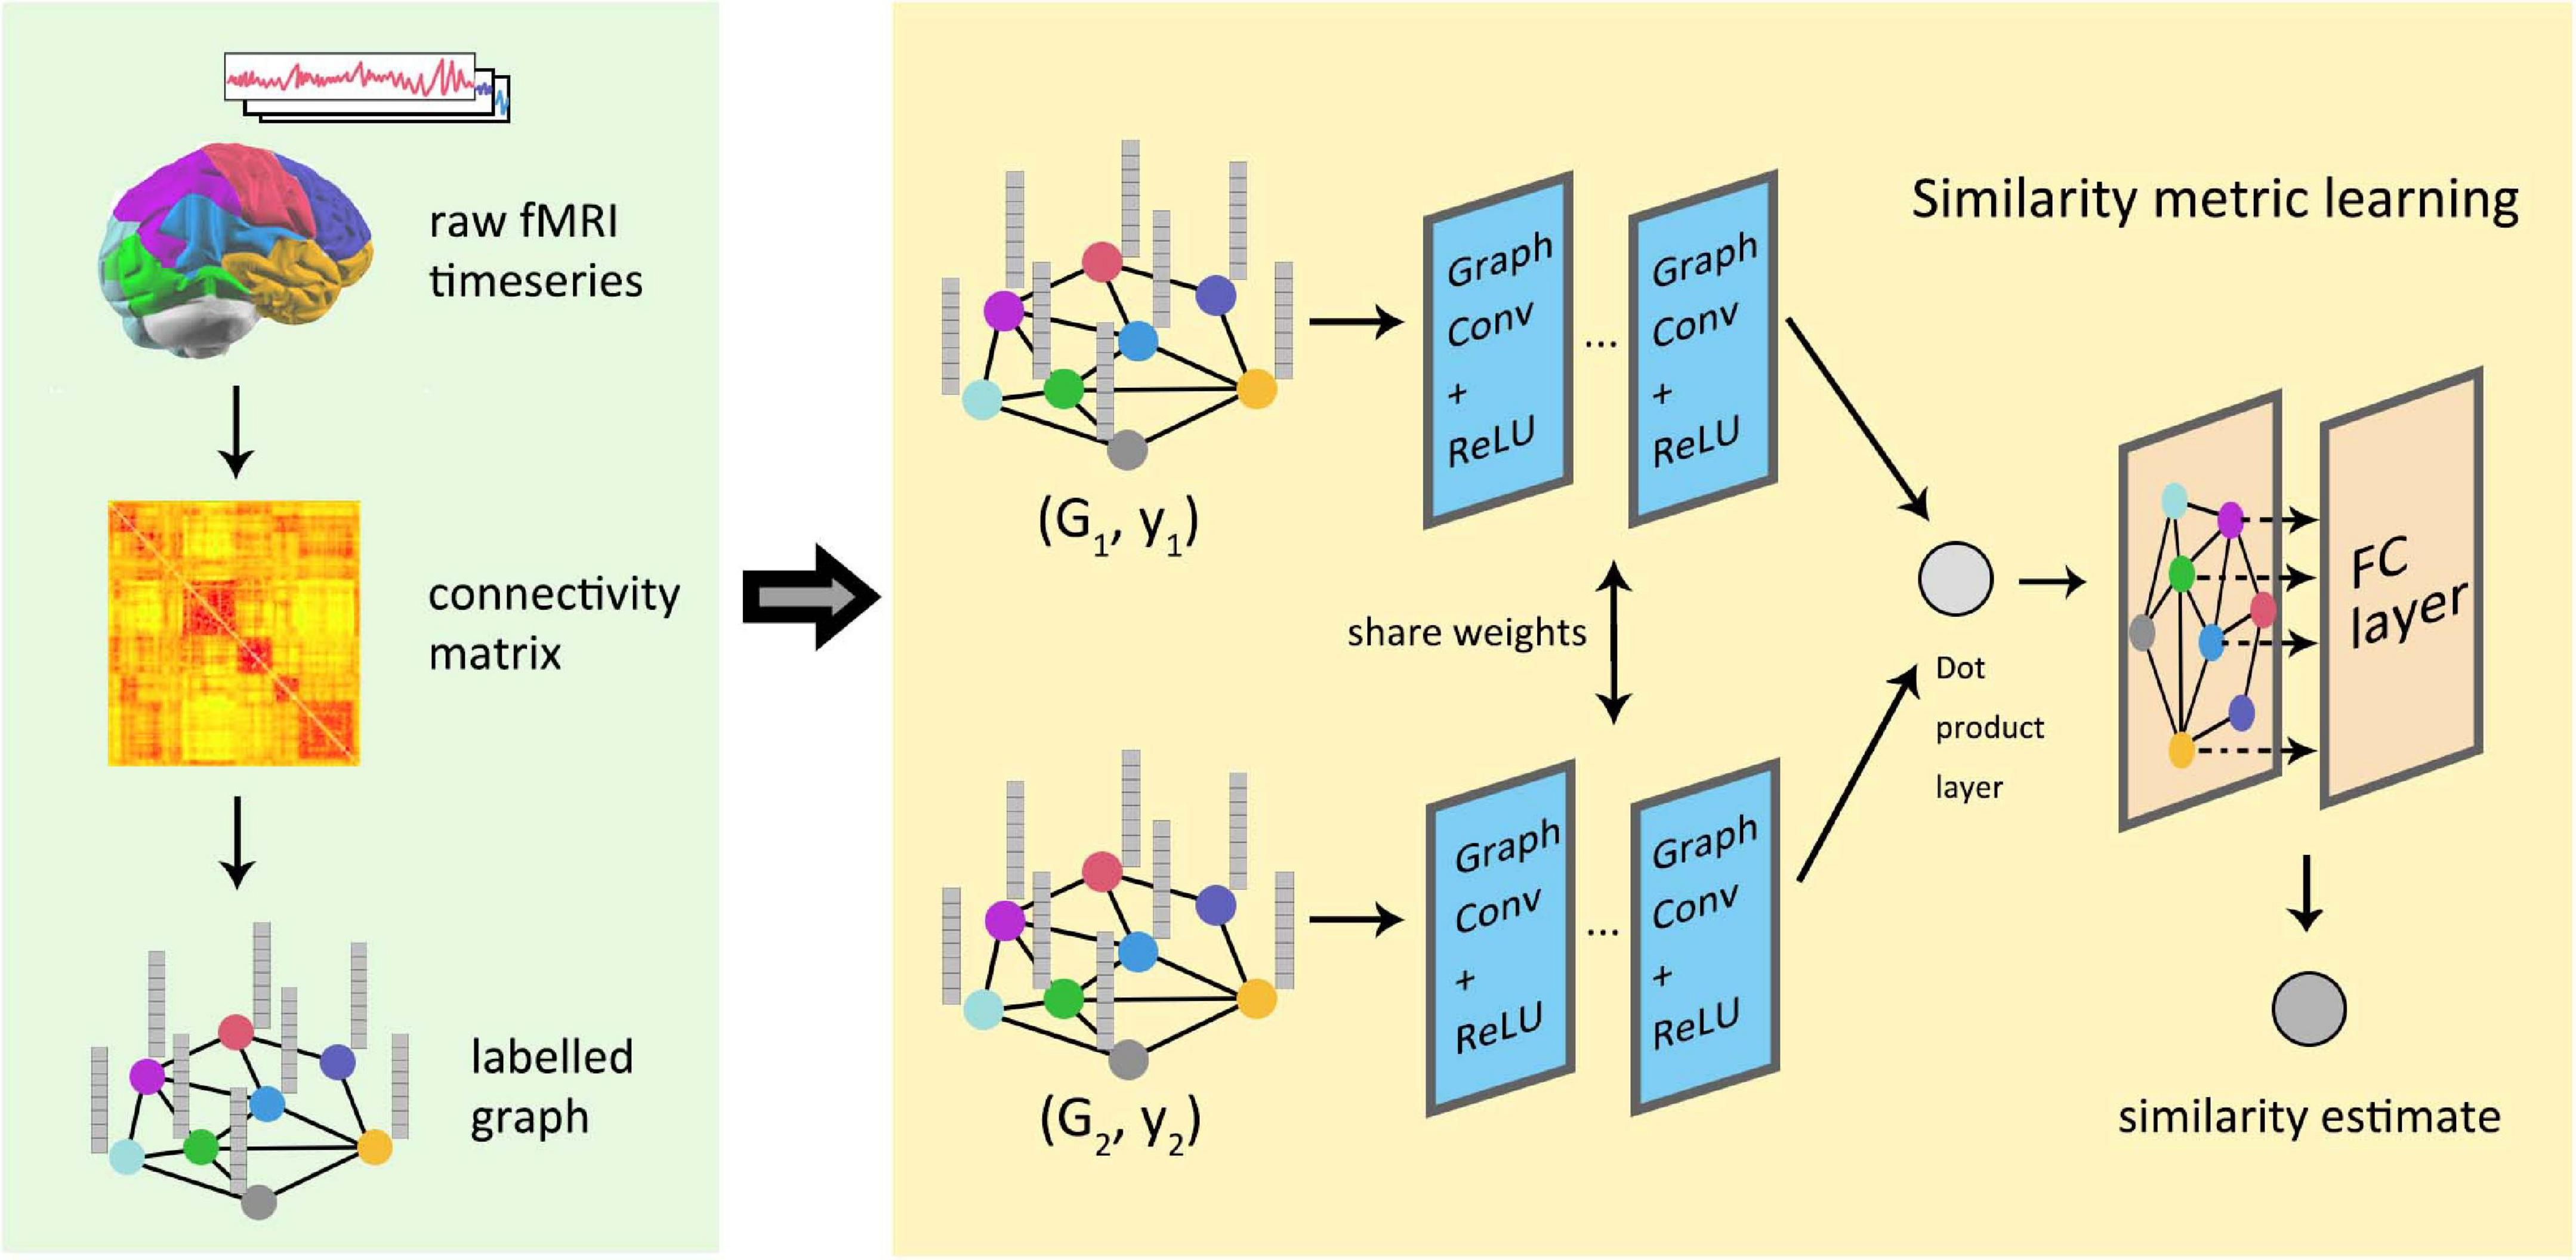
\includegraphics[width= \textwidth]{pics/fgene.jpg}
     \caption{Similarity measure learning of graph neural network in functional brain graphs. The information contained in the fMRI image was integrated into the graph through the graph partition and connection matrix. Two graphs were, respectively, used as the input of the two graph convolutional networks with sharing parameters, and the output of the network was combined by the inner product layer. Finally, a fully connected layer outputs the estimated similarity between the graphs \cite{zhang_graph_2021}}
     \label{fgene}
     %add_ref
\end{figure}

\subsection{Mathematics Behind a GNN}
A single GNN layer consists of two important parts -
\begin{enumerate}
    \item \textbf{Aggregation} - The information from the neighbouring nodes $(N(v))$ us transformed and aggregated. Eg : SUM, MAX, AVERAGE.
    \item \textbf{Update} - The embeddings of the $node (v)$ is updated using the aggregated information from nodes and linearly transformed current node embeddings. Eg : SUM, CONCAT, MLP (Multi Layer Perceptron)
\end{enumerate}

The hidden state of a node at a particular layer $l$ is
\begin{displaymath}
    h_v^{0} = X_v
\end{displaymath}

\begin{displaymath}
    h_v^{(l+1)} = \sigma\Bigl(W_l\sum_{u\in N(v)}\frac{h_u^{(l)}}{|N(v)|} + B_lh_v^{(l)}\Bigr)
\end{displaymath}

The hidden state of all the nodes are transformed using a linear transformation of weight matrix $W_l$ and aggregated using weighted average. 
The current state of the node is also linearly transformed using a weight matrix $B_l$. $\sigma$ is a non linear function, such as the sigmoid function.


\subsection*{Matrix Representation}
Let D be a diagonal matrix where
\begin{displaymath}
   D_{v,v} = Degree(v) = |N(v)|
\end{displaymath}

\begin{displaymath}
    D_{v,v}^{-1} = \frac{1}{|N(v)|}
\end{displaymath}
The term
\begin{displaymath}
    \sum_{u\in N(v)}\frac{h_u^{(l)}}{|N(v)|}
\end{displaymath} 
can be written as
\begin{displaymath}
    D^{-1}AH^{(l)}
\end{displaymath}
Therefore, 
\begin{displaymath}
H^{(l+1)} = \sigma(D^{-1}AH^{(l)}W_l^T + H^{(l)}B_l^T)    
\end{displaymath}

Where $H^{(\ell)}$ is the hidden state matrix at layer $\ell$ and A is the adjacency matrix of the graph. \\ 
The parameters in the weight matrices W and B are tuned by back propagation using MSE (Mean Square Error) or Log Likelihood depending on the ML task.

\begin{displaymath}
\Theta_{\ell,t} = \Theta_{\ell,t-1} - \eta \sum_{i \in \Omega_t} \nabla_i \Theta_{\ell,t-1}    
\end{displaymath}

\subsection{Classification} \label{section_classification}
As a reminder, the GNN layers are used to extract information on how the nodes relate to each other according to our modelling of the problem as a graph. This information is then, commonly, fed into a classification layer.

\begin{figure}
     \centering
     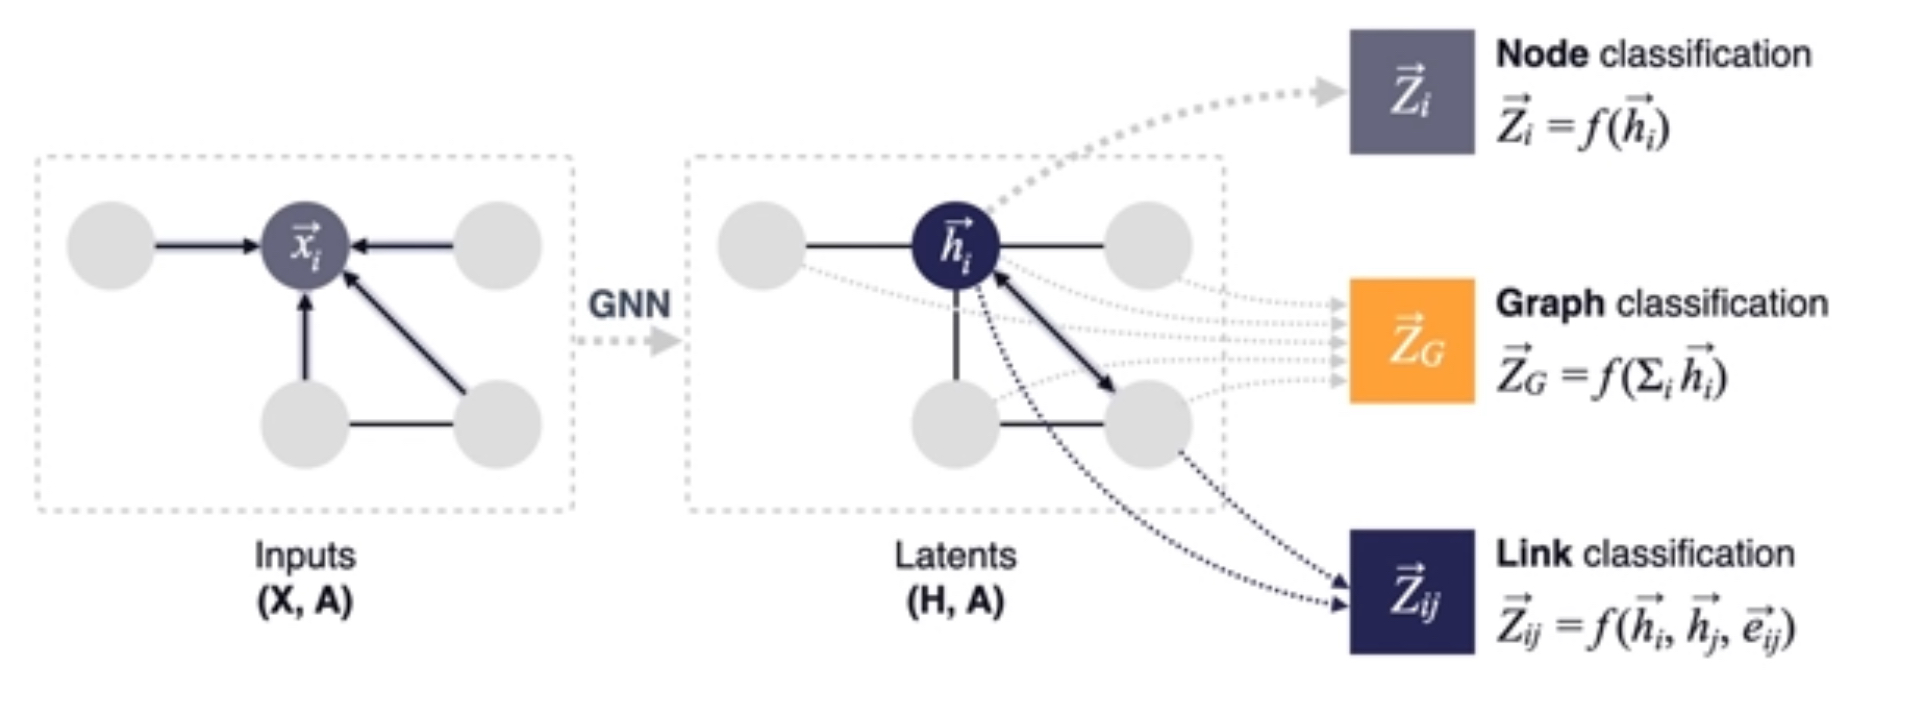
\includegraphics[width= \textwidth]{pics/Classification_Types.jpg}
     \caption{Three Types of GNN Classfication \cite{noauthor_intro_nodate}}
     \label{Classification_Types}
     %add_ref
\end{figure}

Three types of classification exist - 
\begin{enumerate}
    \item Node Classification - here, we try to ascertain what a particular node could be, provided that we have a graph with a good number of nodes labelled
    \item Graph Classification - here, we try to ascertain what the graph as a whole could mean. If we consider an image as a graph, then this would translate to image classification
    \item Link Classification - here, we try to find out if there could be a relationship between two nodes, provided we already have a few links between nodes on the graph
\end{enumerate}

\subsection{General Recipe}
So, the basic recipe for a GNN is
\begin{enumerate}
  %\item Identify the graph structure that you want to apply GNN on i.e, formulate the nodes and edges in the data.
  \item Construct the initial graph structure to model the data as nodes and the relationship between data as edges
  \item Based on the task i.e, node level, edge level as described earlier, create the GNN model's classification layer
  \item Define the loss function according to the context. Eg: log likelihood, root mean square error etc.
  \item Apply gradient descent and optimize the weight parameters by minimizing the loss function
\end{enumerate}